\documentclass{beamer}

\usepackage{minted}
\usepackage{tikz}

\newcommand*\circled[1]{\tikz[baseline=(char.base)]{\node[shape=circle,fill,inner sep=2pt] (char) {\textcolor{white}{#1}};}}


\usepackage[orientation=portrait,size=a1,scale=1.1
]{beamerposter}
\usetheme{JuelichPoster}

\setbeamertemplate{partner1}{
\includegraphics{img/cscs}}
% TODO Add HBP and/or eBrains here

\begin{document}
\begin{frame}[t, fragile]
  \frametitle{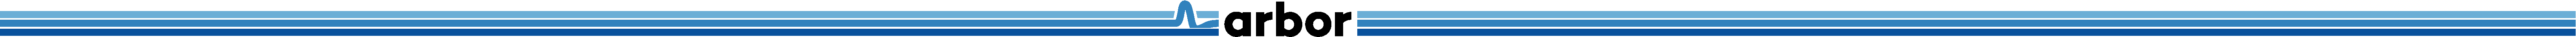
\includegraphics[width=\linewidth]{img/arbor-lines-proto-colour-full}}
  \framesubtitle{A morphologically detailed neural network simulation library for modern high performance computer architectures.\\
    \tiny{Nora Abi Akar, Ben Cumming, Stuart Yates (CSCS); Thorsten Hater, Brent Huisman, Anne Küsters (Forschungszentrum Jülich)}}

  \begin{columns}
    \begin{column}{0.65\textwidth}
      We present recent developments in Arbor, a library for the simulation of
      morphologically detailled neurons and networks thereof. Arbor places strong
      emphasis on performance, portability, and usability. It can exploit modern
      architectures based on super-scalar multi-core processors and GPU accelerators.
      We will showcase some of the features added to Arbor since the last release and
      how they can used to almost directly import single cell models from the Allen
      Brain Atlas database.
    \end{column}
    \begin{column}{0.3\textwidth}
      \begin{block}{Where to find us}
        \begin{description}
          \item[Contact] arbor-sim@fz-juelich.de
          \item[Source code] github.com/arbor-sim/arbor
          \item[Documentation] arbor.readthedocs.io
        \end{description}
      \end{block}
    \end{column}
  \end{columns}

  \begin{appendixblock}
    \begin{minipage}[c]{.48\linewidth}
      \centering
      \color{fzjblue}\rule{0.9\linewidth}{0.2\paperheight}
    \end{minipage}
    \hfill
    \begin{minipage}[c]{.48\linewidth}
    \end{minipage}
  \end{appendixblock}

  \textbf{\structure{Running an Allen Brain Atlas Model}}\\
  \begin{columns}[onlytextwidth]
    \begin{column}{.49\linewidth}
      The code snippet on the right is complete except the parsing and plotting
      steps; it is available in full together with this poster at
      \cite{my-source}. While the electro-physiological data is supplied as a
      JSON file in all instances, the structure as some variation. Thus, the
      parsing cannot be standardised. We comment on some of the important steps
      \begin{itemize}
        \item[\circled{1}] load SWC structure from the download
        \item[\circled{2}] assign labels to geometry
        \item[\circled{3}] build a cell description from labels and geometry
        \item[\circled{4}] parse the electro-physiological properties supplied in the download and assign to regions
        \begin{itemize}
          \item set physical properties: $T$, $V_{m}$, $R_{a}$, $C_{m}$
          \item define ion dynamics reversal potentials
        \end{itemize}
        \item[\circled{5}] Attach to the soma's center
        \begin{itemize}
          \item current clamp; rectangular stimulus of $150\,pA$ from $200\,ms$ to $1200\,ms$
          \item voltage probe; sampling with $200\,kHz$
          \item spike detector; triggering at $V=-40\,mV$
        \end{itemize}
        \item[\circled{6}] convert the cell description into a runnable simulation
        \item[\circled{7}] set mechanism catalogue comprising the defaults and Allen DB mechanisms.
        \item[\circled{8}] run the simulation for $1400\,ms$ with time step $\Delta t = 0.0005\,ms$
      \end{itemize}
      \begin{figure}[H]
        \centering
        \includegraphics{src/arbor.pdf}
        \label{fg:results}
      \end{figure}
      The reference solution was obtained using the allensdk Python package with
      the default Neuron backend \cite{allensdk, neuron}. A minor modification
      was made to suppress editing of the axon at load time of the geometric
      information. For comparable simulations, we instead performed this
      manipulation by hand once and stored the result in the SWC input. We
      observe a minor deviation from the reference run, which is explained by
      different discretisations.

      The elapsed wall clock times for only the simulation steps are $14.7\,s$
      with the code on the right and $121.8\,s$ for the reference solution;
      yielding a speed-up of $8.25\times$ when using Arbor.
    \end{column}
    \begin{column}{.49\linewidth}
      \inputminted[escapeinside=!!]{python}{src/model.py}
    \end{column}
  \end{columns}
\end{frame}
\end{document}
